\label{symbolische-algorithmen}

Bei symbolischen Algorithmen handelt es sich um Methoden zur Lösung von Problemen, indem Daten durch von Menschen interpretierbare Symbole repräsentiert werden und sie durch von Menschen explizit programmierte Regeln verarbeitet werden (\cite{Fergus.2022}, S. 4; \cite{Früh.2022}, S. 5 f.; \cite{Garnelo.2019}).

In diesem Kapitel werden drei symbolische Algorithmen vorgestellt, die verwendet werden können, um in Spielbäumen erfolgversprechende Entscheidungen zu treffen. Zunächst werden die Algorithmen zur Lösung von Spielbäumen Minimax und dessen Optimierung Alpha-Beta-Pruning vorgestellt (\cite{Ferguson.January2019}, Kapitel 4; \cite{Heineman.October2008}, Kapitel 7.6 u. 7.8). Darauf folgt die Erklärung der Monte Carlo Tree Search, welche einen allgemeineren Ansatz darstellt (\cite{Russell.2020}, S. 580; \cite{Swiechowski.2021}).

\subsubsection{Minimax}

Minimax ist ein Algorithmus, der aus Sicht eines Spielers ausgehend von einem beliebigen Ursprungsknoten im Spielbaum die darauf folgenden Knoten bewertet und den Kindknoten des Ursprungsknotens mit der besten Bewertung zurückgibt. Bei der Bewertung wird davon ausgegangen, dass der Gegner ebenfalls den Zug wählt, der für ihn am günstigsten ist. Der zu untersuchende Spieler versucht, die Bewertung zu maximieren, während der Gegenspieler versucht, sie zu minimieren.

Zunächst werden die Blattknoten des Spielbaums bewertet. Je günstiger ein Spielfeldzustand für den zu untersuchenden Spieler ist, desto größer ist die Zahl, die diesem Zustand zugeordnet wird. In Abhängigkeit der zuvor bewerteten Knoten, werden nun deren Elternknoten bewertet. Ist im betrachteten Zustand der zu untersuchende Spieler am Zug, übernimmt der Elternknoten die Bewertung des Kindknotens mit der höchsten Bewertung. Umgekehrt ist es, wenn der Gegenspieler Spieler am Zug ist. Dann bekommt der zu untersuchte Knoten die Bewertung des Kindknotens mit der niedrigsten Bewertung. Dieser Vorgang wird wiederholt, bis der Ursprungsknoten erreicht ist. Zurückgegeben wird der Kindknoten des Ursprungsknotens, dem die größte Bewertung zugeordnet wurde.

Erfolgt die Bewertung anhand der Gewinnchancen, führt das dazu, dass die Wahl des Knotens mit der besten Bewertung auch die Gewinnchancen maximiert. Um die Gewinnchancen zu ermitteln, müssen jedoch alle Knoten des Spielbaums untersucht werden. Die Laufzeit des Algorithmus steigt linear zur Anzahl der zu untersuchenden Knoten und damit bei konstanter Anzahl von Möglichkeiten pro Zug exponentiell zur Suchtiefe. Den gesamten Spielbaum zu durchsuchen, ist daher nur für wenig komplexe Spiele praktikabel. Damit die Bewertung in akzeptabler Zeit erfolgen kann, muss für komplexere Spiele die Suchtiefe oder -breite begrenzt werden und die Bewertung der Knoten muss auf Grundlage von Heuristiken erfolgen (\cite{Ferguson.January2019}, Kapitel 4; \cite{Heineman.October2008}, Kapitel 7.6).

\subsubsection{Alpha-Beta-Pruning}

Beim Alpha-Beta-Pruning handelt es sich um eine Optimierung des Minimax-Algorithmus. Dabei werden die Teilbäume übersprungen, die bei optimaler Spielweise beider Spieler nicht erreicht werden, und damit das Ergebnis nicht beeinflussen können. Alpha-Beta-Pruning liefert dieselben Ergebnisse wie der Minimax-Algorithmus, aber untersucht dabei wesentlich weniger Knoten im Spielbaum.

Dazu werden während der Suche die Werte Alpha und Beta aufgezeichnet. Alpha entspricht der Mindestbewertung, die der zu untersuchende Spieler garantieren kann, wenn beide Spieler optimal spielen. Beta entspricht der Bewertung, die der Gegenspieler bei optimaler Spielweise maximal zulassen wird. Zu Beginn der Suche wird Alpha auf minus unendlich und Beta auf plus unendlich initialisiert.

Alpha wird aktualisiert, wenn für einen Knoten, bei dem der zu untersuchende Spieler am Zug ist, ein Kindknoten gefunden wurde, dessen Bewertung größer ist als das bisherige Alpha. Beta hingegen wird aktualisiert, wenn für einen Knoten, bei dem der Gegenspieler am Zug ist, ein Kindknoten gefunden wurde, dessen Bewertung kleiner ist als Beta.

Sobald bei einem Knoten Alpha größer oder gleich Beta ist, kann die Untersuchung dessen Kindknoten aus folgenden Gründen abgebrochen werden:

\begin{itemize}
	\item Ist bei diesem Knoten der zu untersuchende Spieler am Zug, hatte der Gegenspieler in einem zuvor untersuchten Teilbaum bessere Chancen, und wird den aktuellen untersuchten Teilbaum nicht auswählen.
	\item Ist bei diesem Knoten der zu Gegenspieler am Zug, hatte der zu untersuchende Spieler in eine zuvor untersuchten Teilbaum bessere Chancen, und wird den aktuell untersuchten Teilbaum nicht auswählen (\cite{Heineman.October2008}, Kapitel 7.8; \cite{Ferguson.January2019}, Kapitel 4.5).
\end{itemize}

So kann im Vergleich zum Minimax-Algorithmus die Untersuchung von 80\% bis 95\% der Knoten übersprungen werden. Der Anteil der Knoten, die bei der Untersuchung übersprungen werden können, ist abhängig davon, wie schnell das Fenster zwischen Alpha und Beta verkleinert wird. Wenn die Reihenfolge, in der die Züge untersucht werden, geschickt gewählt wird, kann dies sogar zu einer Reduktion von über 99\% führen (\cite{Heineman.October2008}, Kapitel 7.8). In Schach ist dies beispielsweise möglich, indem Züge früher bewertet werden, je höherwertiger eine im Zug geworfene Figur ist.

Durch Alpha-Beta-Pruning kann der Spielbaum bei gleichbleibender Zeit wesentlich tiefer durchsucht werden, was beim Einsatz von Heuristiken als Bewertungsfunktion zu präziseren Ergebnissen führt. Die Laufzeit ist allerdings weiterhin exponentiell abhängig zur Suchtiefe. Den gesamten Spielbaum zu durchsuchen, um die Bewertung auf Grundlage von tatsächlichen Gewinnaussichten durchzuführen, bleibt bei komplexeren Spielen weiterhin unpraktikabel (\cite{Heineman.October2008}, Kapitel 7.8).

Heuristische Bewertungsfunktionen sind im Rahmen dieser Arbeit in der Hinsicht problematisch, als dass sie spezifisch für die Regeln eines Spiels zugeschnitten sein müssen, bzw. dass es für bestimmte Anwendungsfälle keine guten Heuristiken gibt (\cite{Ferguson.January2019}, Kapitel 4.5). Das führt dazu, dass die Eigenschaften von Alpha-Beta-Pruning schwer auf verschiedene Anwendungsfälle übertragbar sind.

\subsubsection{Monte Carlo Tree Search}

Bei Monte Carlo Tree Search (MCTS) handelt es sich um einen heuristischen Algorithmus, der dazu dient, um in Bäumen, die aus sequentiellen Entscheidungen bestehen, einen möglichst vielversprechenden Pfad auszuwählen. MCTS kann als Lösung für MDPs betrachtet werden (\cite{Russell.2020}, S. 580). Dazu werden wiederholt zufällig verschiedene Entscheidungen simuliert und deren potentieller Erfolg statistisch ausgewertet.

Der Vorteil gegenüber des Alpha-Beta-Prunings besteht darin, dass es bei MCTS nicht notwendig ist, innere Knoten, also Nicht-Blattknoten, zu bewerten (\cite{Russell.2020}; \cite{Ferguson.January2019}; \cite{Browne.2012}). Lediglich die Endzustände müssen bewertet werden können. Dies lässt sich im Gegensatz zur Bewertung von inneren Knoten relativ einfach umsetzen. Bei Spielen bedeutet das die Auswertung des Endergebnisses, wie zum Beispiel den Gewinner oder eine Punktzahl (\cite{Russell.2020}, S. 161; \cite{Ferguson.January2019}, Kapitel 4.5; \cite{Browne.2012}).

MCTS ist eine weit verbreitete Lösung für kombinatorische Spiele und hat sich insbesondere beim Spiel Go als erfolgreich bewiesen, das einen besonders breiten und tiefen Spielbaum aufweist, woran frühere Verfahren gescheitert sind. Der Algorithmus wird auch abseits von Spielen in verschiedenen Variationen eingesetzt, so zum Beispiel in der Optimierung von Lieferketten und der Zeitplanung von Prozessen (\cite{Russell.2020}, S. 161; \cite{Browne.2012}).

% Funktionsweise

Mit MCTS werden Entscheidungsmöglichkeiten statistisch ausgewertet, indem die in Abbildung \ref{fig:f27} dargestellten vier Phasen Selection, Expansion, Simulation (auch Play-Out) und Backpropagation wiederholt durchlaufen werden. Dabei wird ein Baum verwaltet, der eine ähnliche Struktur wie der Spielbaum aufweist. Die Knoten beschreiben die Zustände der Umgebung und die Kanten Übergänge zwischen den Zuständen. Zu jedem Knoten im MCTS-Baum wird eine Statistik abgespeichert, die Informationen darüber enthält, wie oft der Knoten selbst oder dessen Kindknoten die Simulation-Phase durchlaufen haben, und was die Ergebnisse der Simulationen waren (\cite{Russell.2020}, S. 161 ff.; \cite{Ferguson.January2019}, Kapitel 4.5).

\begin{figure}[ht!]%[!tbp]
	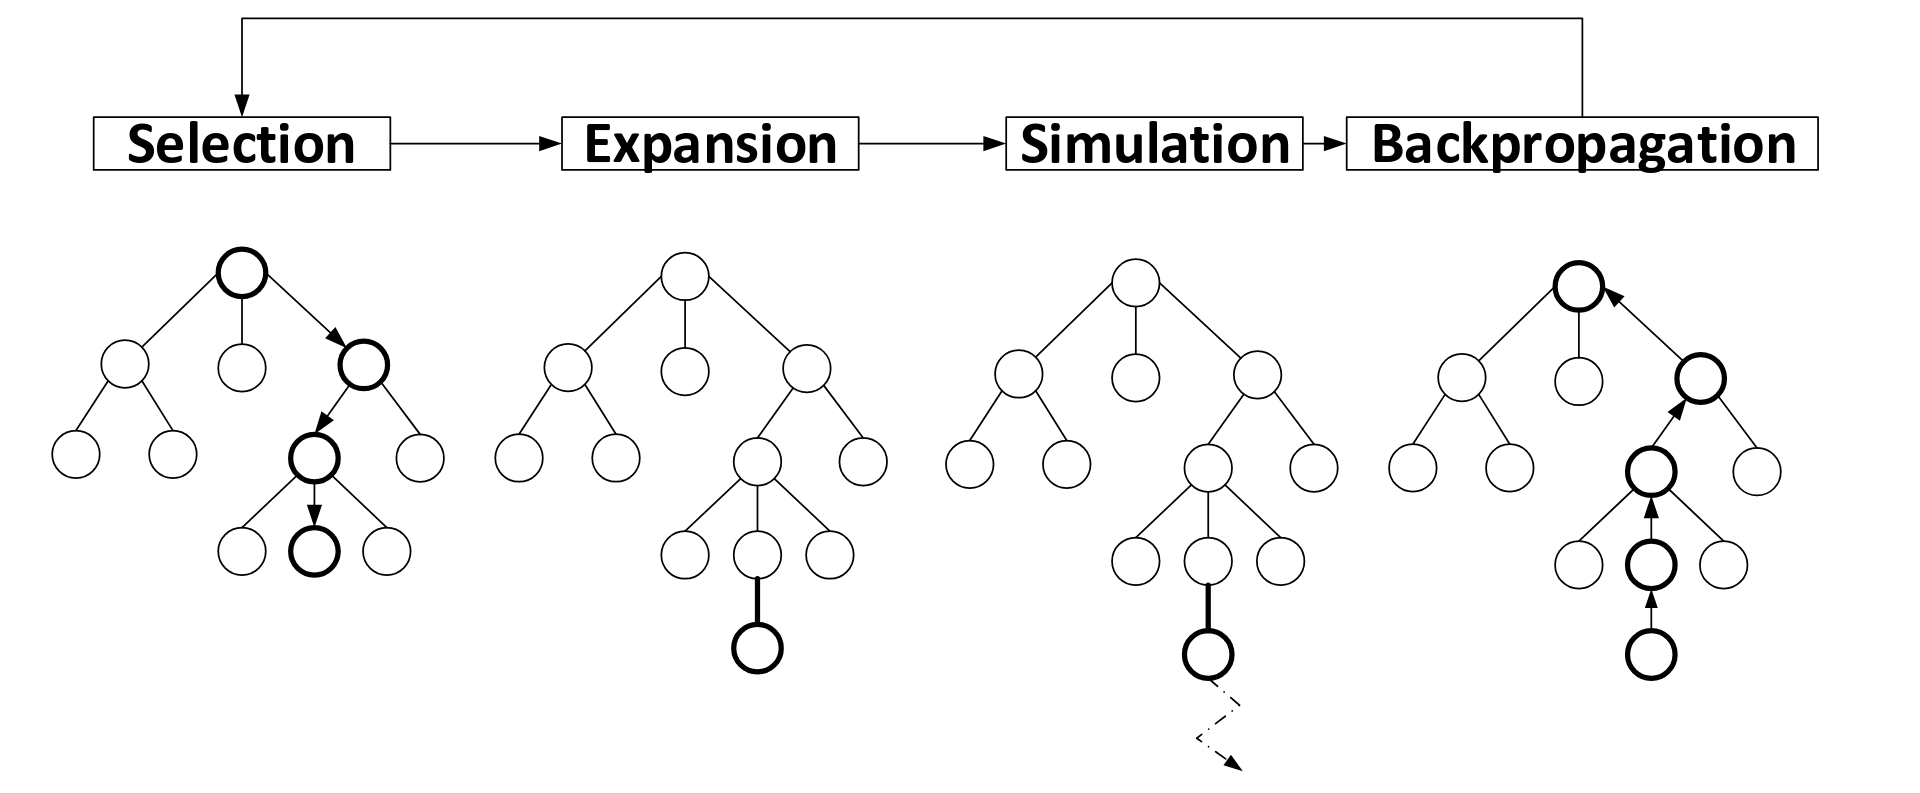
\includegraphics[width=0.8\textwidth, center]{Bilder/mcts-phases.png}
	\caption[Die vier Phasen des MCTS-Algorithmus.]{Die vier Phasen des MCTS-Algorithmus \cite{Swiechowski.2021}.}
	\label{fig:f27}
\end{figure}

Zu Beginn besteht der MCTS-Baum lediglich aus dem Ursprungsknoten. In der Phase \textbf{Selection} wird zunächst der Ursprungsknoten aus dem MCTS-Baum betrachtet und es werden basierend auf den bisher gesammelten Statistiken so lange Folgeknoten gewählt, bis ein Knoten erreicht wird, der um mindestens einen Folgeknoten erweitert werden kann. Dieser Knoten wird in den noch kommenden Phasen untersucht. Dabei besteht jeweils die Möglichkeit, einen Knoten zu wählen, der vielversprechend erscheint, um genauere Informationen darüber zu erhalten (Exploitation), oder einen Knoten zu wählen, der noch nicht so oft untersucht wurde, um neue Bereiche im Spielbaum mit ggf. besseren Chancen zu erkunden (Exploration). Es gibt verschiedene Auswahlstrategien, wobei UCT (Upper Confidence Bound applied for Trees) die am weitesten verbreitete ist. Dabei wird die UCB1-Formel (\ref{uct-formula}) eingesetzt, die ursprünglich zur Lösung von Bandit-Problemen (vgl. \cite{Russell.2020}, S. 581 ff.) konzipiert wurde, um die Kinder eines Knotens $n$ zu bewerten. Anschließend wird der Knoten mit der höchsten Bewertung gewählt (\cite{Kocsis.2006}; \cite{Browne.2012}; \cite{Russell.2020}, S. 163).

\begin{equation}\label{uct-formula}
	UCT = \frac{U(n)}{N(n)} + c_{UCT} \cdot \sqrt{\frac{log(N(Parent(n)))}{N(n)}}
\end{equation}

Dabei ist $U(n)$ der summierte Wert der Ergebnisse der bisher durchgeführten Simulationen ab Knoten $n$. In Vier Gewinnt entspricht das der Anzahl, wie oft der zu untersuchende Spieler in den bisher durchgeführten Simulationen gewonnen hat. $N(n)$ entspricht der Anzahl der Simulationen, die bisher ab Knoten $n$ durchgeführt wurden. Damit stellt der Term $\frac{U(n)}{N(n)}$ den Exploitation-Teil dar. Er wächst mit den Erfolgsaussichten des untersuchten Knotens.
$N(Parent(n))$ ist die Anzahl der Simulationen des Elternknotens von $n$. Der Term $\sqrt{\frac{log(N(Parent(n)))}{N(n)}}$ wird größer, je seltener ein Knoten simuliert wurde und fördert damit die Exploration von bisher selten untersuchten Knoten.
Bei $c_{UCT}$ handelt es sich um einen Parameter, über den die Exploitation- und Exploration-Teile der Formel ausbalanciert werden können. Als Richtwert wird hier $\sqrt{2}$ empfohlen (\cite{Russell.2020}, S. 163).

Im Zuge der \textbf{Expansion} wird vom zuvor ausgewählten Knoten ein zufälliger Zug ausgeführt und der neue Zustand wird als Kindknoten hinzugefügt. Je nach Spielfeldzustand handelt es sich beim neuen Zug um einen Zug des zu untersuchenden Spielers oder des Gegenspielers. Es können auch mehrere oder alle möglichen Züge auf einmal ausgeführt und als Kindknoten hinzugefügt werden, wenn die durchschnittliche Anzahl der Kindknoten und die verfügbaren Rechenressourcen dies zulassen (\cite{Russell.2020}, S. 162; \cite{Browne.2012}).

In der \textbf{Simulation}-Phase werden ab den zuvor hinzugefügten Knoten so oft zufällige Entscheidungen hintereinander simuliert, bis ein Endzustand erreicht wurde. Es ist dabei zu beachten, dass die getroffenen Entscheidungen nicht in den MCTS-Baum aufgenommen werden (\cite{Russell.2020}, S. 162). Besteht eine Simulation aus besonders vielen Zügen, kann es sinnvoll sein, sie nach einer bestimmten Anzahl von Zügen abzubrechen. Der letzte erreichte Zustand kann dann heuristisch oder mit einem neutralen Ergebnis bewertet werden (\cite{Russell.2020}, S. 164). Es existiert eine Variante, die sogenannte Heavy-Playouts einsetzt, was bedeutet, dass die Entscheidungen in der Simulation nicht rein zufällig getroffen werden, sondern unter Zuhilfenahme von Wissen über das konkret zu lösende Problem. Dadurch werden die Simulationen realistischer \cite{Browne.2012}.

Als letztes erfolgt die Phase \textbf{Backpropagation}. Das Ergebnis der Simulation wird für den untersuchten Knoten im MCTS-Baum abgespeichert und die Statistik der Knoten, die vom Ursprungsknoten zum untersuchten Knoten geführt haben, wird aktualisiert. Zurückgegeben wird der Folgeknoten des Ursprungsknoten, der am häufigsten besucht wurde (\cite{Russell.2020}, S. 162).

Mit jeder Wiederholung der vier Phasen wird die Statistik über die Erfolgschancen der Entscheidungsmöglichkeiten akkurater. Nach einer bestimmten Anzahl von Wiederholungen wird basierend auf den gesammelten Statistiken eine Entscheidung getroffen.

Da die Phasen Expansion und Simulation basierend auf Zufall erfolgen, ist MCTS nicht deterministisch und liefert keine perfekten Vorhersagen. Außerdem besteht vor allem bei wenigen Iterationen die Gefahr, dass wenige kritische Züge unentdeckt bleiben, und die Statistik inakkurat wird (\cite{Russell.2020}, S. 164).

Die Laufzeit von MCTS ist schwer mit den zuvor genannten Methoden vergleichbar, da die Iterationen beliebig oft durchgeführt werden können, um die Vorhersagen zu verbessern. Durch Untersuchungen wurde gezeigt, dass bei kleinen Problemen und der Verfügbarkeit von präzisen Heuristiken Alpha Beta mit begrenzter Suchtiefe schneller und besser arbeitet. MCTS schneidet im Vergleich besser ab, je tiefer und stärker verzweigt die zu lösenden Entscheidungsbäume sind (\cite{Russell.2020}, S. 163 f.). Es wurde außerdem gezeigt, dass die Ergebnisse von MCTS unter Verwendung der UCT als Selection-Strategie bei unbegrenzten Ressourcen zu Minimax konvergiert \cite{Browne.2012}.

Es existieren verschiedene Variationen und Verbesserungen für die Strategien in den Phasen Selection und Expansion, die unter bestimmten Umständen für bessere Vorhersagen sorgen. Dazu gehören auch welche, die Machine Learning einsetzen, um in der Selection-Phase fundiertere Entscheidungen zu treffen \cite{Browne.2012}. Diese werden im Rahmen dieser Arbeit nicht betrachtet. MCTS soll hier klar von Machine-Learning-Verfahren abgegrenzt sein. Es wird davon ausgegangen, dass die Verbesserungen für die Untersuchung der Robustheit nicht relevant sind und dass sich die Beobachtungen auch auf Varianten von MCTS übertragen lassen.
